\documentclass{article}
\usepackage[utf8]{inputenc}
\usepackage{amsmath}
\usepackage{float}
\usepackage{multicol}
\usepackage{natbib}
\usepackage{graphicx}
\usepackage{breqn}
\usepackage{amsmath}
\usepackage{titlesec}
\usepackage{enumerate}
\usepackage{color, colortbl}
\usepackage{algorithm}
\usepackage{algorithmic}
\usepackage{algorithm2e}
\usepackage{algpseudocode}
\usepackage{tikz,pgfplots}
\definecolor{Gray}{gray}{0.9}
\setlength{\columnsep}{0.8cm}
\setlength{\parindent}{0cm}
\newtheorem{theorem}{Theorem}
\newtheorem{lemma}{Lemma}
\newtheorem{definition}{Definition}

\title{A randomized scheme for Cuts and Flows in Capacitated Graphs}
\author{    Jiang Chunhui \\ \texttt{A0162518E} \and
            Wang Junming \\ \texttt{A0162553H} }
\date{April 2019}

\usepackage{natbib}
\usepackage{graphicx}

\begin{document}

\maketitle

\section{Introduction}
A cut is a partition of vertices into two disjoint non-empty sets. The value of the cut is the number of edges across the cut or the total weight of edges across the cut for the weighted graph. Intuitively, the minimum cut is the cut with minimum value. Similarly, an s-t min cut is a cut with the additional constraint that node s and t has to be on the opposite side. It has been shown in \citep{karger1999random} that random sampling can be used to approximate the value of cuts in the graph. The idea is to construct a skeleton graph by sampling each edge with a certain probability, producing a sparser sampled graph that can approximate all cut values of the original graph correctly with high probability.

\begin{figure}[h!]
\centering
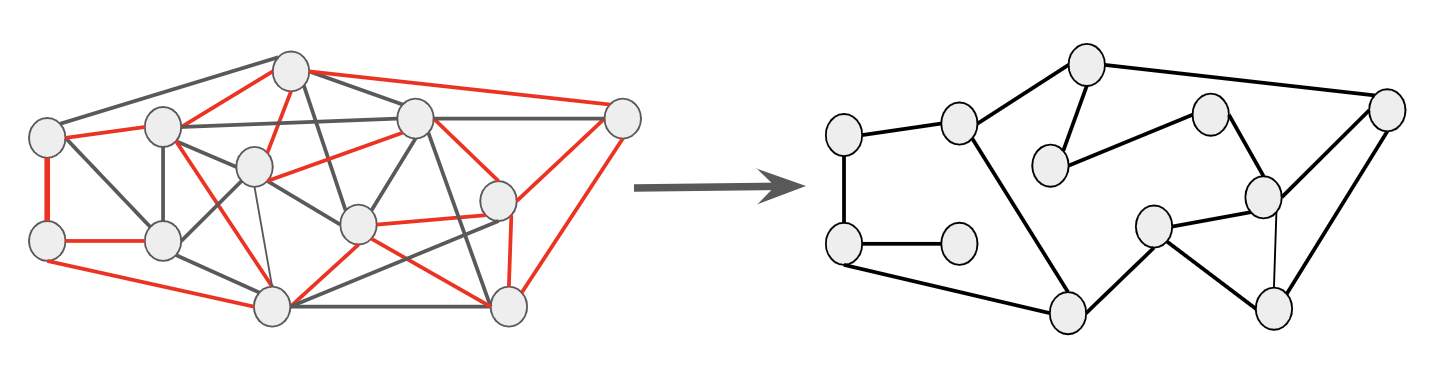
\includegraphics[scale=0.4]{images/sample.png}
\caption{Sampling}
\label{fig:sampling}
\end{figure}

More specifically, we sample each edge with probability $p = \theta (\frac{\ln{n}}{\epsilon^2c})$, where c is the value of min-cut in the graph, such that with high probability, each s-t min cut in the graph has value between $(1-\epsilon)pv$ and $(1+\epsilon)pv$. Given the skeleton graph has less number of edges, we can run our classic max-flow algorithm faster to achieve an approximation of the original cut. One limitation of such an approach is that the sampling probability depends on the value of the minimum cut. Thus when the minimum cut is small, we cannot make many improvements, that is, the resulting skeleton graph is still dense. However, it has been later shown in \citep{benczur2015randomized} that we can use nonuniform sampling to remove the dependency on the minimum cut value c, such that the skeleton graph will have O(nlogn) number of edges regardless the value of the minimum cut. The basic idea is to decompose the graph into dense and sparse parts and sampling them with a different probability. In order to identify dense sub-component of the graph, a new definition edge strength is introduced, which is the maximum value k such that a sub-graph of minimum cut k contains this edge. which we will formally define in section 3. One open question the author has proposed is whether we can use standard edge connectivity to replace edge strength in the non-uniform sampling scheme. Where standard edge connectivity of an edge is the minimum value of a cut separating the endpoints of the edge. We have done a series of experiment to answer this question, the details can be found in section 4.

In this paper, we will first revisit the uniform sampling scheme with dependency on the minimum cut value c as introduced in \citep{karger1999random}, followed by a divide-and-conquer algorithm to find exact s-t max-flow inspired by the idea of uniform sampling. We will then introduce a non-uniform sampling scheme as introduced in \citep{benczur2015randomized} to remove graph sampling's dependence on the minimum cut value, followed by showing how can we estimate edge strength effectively. Lastly, our first extension will be based on an open question proposed by the authors: can we use standard connectivity instead of strong connectivity in the non-uniform sampling scheme. We will run experiments on several typical graphs and analyze their performance. Furthermore, we will propose a streaming algorithm to update the skeleton graph without the knowledge of the original graph, based on the assumption that using standard connectivity still yields good sampling. 

\section{A Uniform Sampling Scheme}

\subsection{Basic Method}

Consider an unweighted graph $G$ with n vertices and m edges, with minimum cut size c. We want to sample each edge with some probability $p_e$, producing a sampled graph much sparser than original, but all cuts in the sampled graph deviate from the expected value by no more than a factor of $\epsilon$. For a cut of value $\alpha c$, where $\alpha \geq 1$, we can use Chernoff bound to show the probability of not deviating by a factor of $\epsilon$ from expected:

\begin{equation}
    Pr[|X - p_e\alpha c| > \epsilon p_e\alpha c] \leq 2e^{-\epsilon^2p_e\alpha c/3}
\end{equation}

Naturally, the next step is to take a union bound over all cuts, get the probability that all cuts does not deviate from expected by a factor of $\epsilon$. Intuitively, cuts of small value have a larger probability of going wrong. However, we have the following lemma to bound the number of cuts of small value. 

\begin{lemma}[Karger \cite{karger1999random}] \label{boundcuts}
In an undirected graph with minimum cut value c, the number of cuts of value less than $\alpha c$ is less than $n^{2\alpha}$.
\end{lemma}

We can now bound the probability by assuming the worst case scenario (take equality of above lemma). Let $f(\alpha)$ be the number of cuts of value $\alpha c$. Thus taking a union bound, the probability $P$ that no cut deviates by a factor of $\epsilon$ will be:

\begin{equation}
    P \leq f(\alpha) * 2e^{-\epsilon^2p_e\alpha c/3}
\end{equation}

With Lemma \ref{boundcuts} and take the equality sign by assuming worst case scenario, we have $F(x) = \int_{1}^{x} f(\alpha) d\alpha = n^{2x}$, thus $f(x) = \frac{dF}{d\alpha} = \frac{dn^{2x}}{d\alpha}$. 
After working out the math, wo have the following theorem:
\begin{theorem}[Karger \cite{karger1999random}] \label{theorem1}
In an undirected, unweighted graph with minimum cut value c, if we sample each edge with probability $p = \theta (\frac{\ln{n}}{\epsilon^2c})$, every cut in sampled graph will be $(1 \pm \epsilon)$-approximate to the expected cut size with high probability.
\end{theorem}

Notice in order to do the sampling, the knowledge of minimum cut value c is required. We can use Matula's linear time minimum cut algorithm to find a 3-approximation. Overestimation of minimum cut value only makes the sampling probability larger, thus we can still get the right estimation with high probability. Furthermore, since it is a constant factor approximation, the expected number of edges to be sampled will remain in the same order.
\bigskip

The sampling probability is related to the minimum cut value of original graph, thus when the minimum cut value is small, we might not be able to reduce many edges, even though the original graph is overall dense. We will introduce a non-uniform sampling scheme to remove the dependency on the minimum cut value in section 3.

\subsection{Applications}

\subsubsection{Approximating s-t min cut\citep{karger1999random} }
One straight-forward application to the above sampling scheme is to approximate an arbitrary s-t min cut of the original graph. 
We simply applying the sampling scheme described above, choose each edge with probability $p = \theta (\frac{\ln{n}}{\epsilon^2c})$.
After constructing the skeleton graph, we apply the classic augmenting path algorithm for maximum flows to find the s-t maximum flow value $\hat{v}$ of the skeleton graph.
By Theorem \ref{theorem1}, $\hat{v}/p$ gives us a $(1 + \epsilon)$ approximation of the s-t min cut value in the original graph with high probability.
Recall that the augmenting path algorithm finds max-flow(min-cut by duality) in $O(mv)$ where $m$ is the number of edges and $v$ is the value of maximum-flow.
Thus, running this algorithm in skeleton graph results in running time of $O((pm)(pv)) = O(mv\ln^2{n}/\epsilon^4c^2)$

\subsubsection{Find Exact s-t Min Cut\citep{karger1999random}}
A more interesting application is to find the exact s-t max-flow(min-cut) with a randomized divide and conquer approach. The basic algorithm is as follows:

\begin{enumerate}
  \item Split graph $G$ into two sub-graphs $G_1$ and $G_2$, each preserves all vertices in $G$, and each edge is put into $G_1$ or $G_2$ with probability 1/2.
  \item Run the algorithm recursively on $G_1$ and $G_2$ to find s-t max-flow on the two sub-graphs.
  \item Adding up the two cuts, yielding an s-t flow for $G$ (not necessarily maximal).
  \item Continue running augmenting path algorithm on the s-t flow until reach maximum. 
\end{enumerate}

Notice after merging the two s-t flows of $G_1$ and $G_2$, we get an s-t flow of original graph $G$, the idea is to bound the value of the s-t flow in expectation by Theorem \ref{theorem1} to show that with high probability, the value of the flow is not too far from the maximum, such that the augmenting algorithm can run efficiently.
Formally, if we consider sub-graphs $G_1$ and $G_2$ as sampled graph with sampling probability 1/2. Then we can apply Theorem \ref{theorem1}, with $p = 1/2$, thus $\epsilon = \sqrt{2=\log n / c}$, it follows that with high probability, the s-t maximum flow in $G_1$ or $G_2$ has value at least $v(1-1/\sqrt{c})/2$, and the minimum cut value of $G_1$ is $c(1-1/\sqrt{c})/2 = \theta(c)$. Then the merged s-t flow has value $v - \hat{O}(v/\sqrt{c})$ with high probability. Thus in expectation we only need to perform $\hat{O}(v/\sqrt{c})$ augmentations to reach the maximum. As such, the running time of the algorithm will be:

\begin{equation}
T(m, v, c) = 2T(m/2, v/2, c/2) + \hat{O}(mv/\sqrt{c})
\end{equation}

Solve the above recurrence equation, we get expected running time of $\hat{O}(mv/\sqrt{c})$. We have improved the running time by a factor of $1/\sqrt{c}$, while we cannot get much improvement if the minimum cut value of the original graph is small.

\section{A Non-Uniform Sampling Scheme}
Recall that the sampling probability $p$ in uniform sampling scheme is $p = \theta (\frac{\ln{n}}{\epsilon^2c}) = \Omega(\frac{1}{c})$. A limitation of the uniform sampling is that the sampling probability only depends on the minimum cut size $c$ of the original graph. 
Note that one of our purposes for sampling is to reduce the number of edges so that subsequent graph algorithms will run faster.
However, consider a graph with a large number of edges but small min-cut.

For example, in figure \ref{fig:dense_spase}, although the sub-graph in the red circle is dense, the minimum cut size of the whole graph is $1$. The sampling probability based on a minimum cut will be high in this case, and we may not remove many edges from the dense part.

\begin{figure}[h!]
\centering
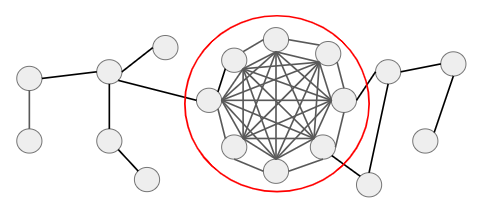
\includegraphics[scale=0.4]{images/dense_sparse_graph.png}
\caption{An Example that Uniform Sampling Performs Poorly}
\label{fig:dense_spase}
\end{figure}

Note that the graph on which uniform sampling does not work well has a pattern: some sub-graphs of it are very dense while other sub-graphs are sparse. In \cite{benczur2015randomized}, Karger et al proposed to sampling the dense sub-graphs and sparse sub-graphs separately with different probabilities. 

As shown in figure \ref{fig:separate_graph}, we split the original graph into two components, and sample each component with probability based on its minimum cut size. Then the dense component will have low sampling probability, which can remove many edges. Finally, combining the two components after sampling will give us a relatively good result.

\begin{figure}[h!]
\centering
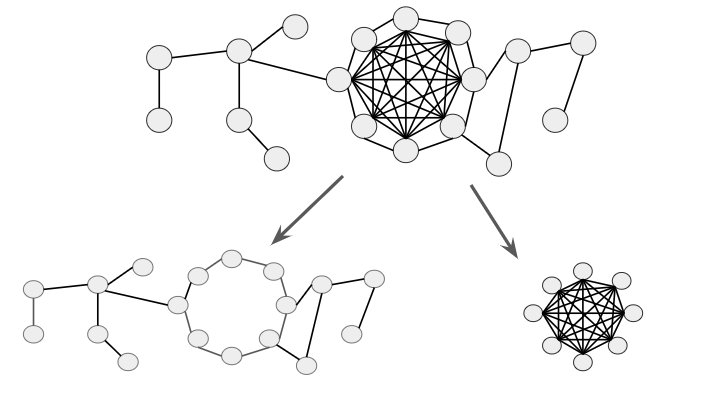
\includegraphics[scale=0.4]{images/separate_graph.png}
\caption{Separate Graph for Sampling}
\label{fig:separate_graph}
\end{figure}

Typically, let $\rho = O(\log n)$. Consider a graph $G$ with minimum cut size $c$, and it has a dense sub-graph $K$ with connectivity $k$. 
During the sampling, for each edge in $K$, we assign weight $\frac{k}{\rho}$ to it and sampling it with probability $\frac{\rho}{k}$. On the other hand, for each edge in $G-K$, we assign weight $\frac{c}{\rho}$ to it and sampling it with probability $\frac{\rho}{c}$. This makes the expected value of each edge to be exactly 1.
This process will not affect the conclusion derived by uniform sampling. For an edge in $K$, we can decompose it as two edges: one with weight $\frac{c}{\rho}$ and another with weight $\frac{k-c}{\rho}$. 
Then, the original graph $G$ can be viewed as two graphs $G_1$ and $G_2$. $G_1$ has same vertices and edges as $G$, with each edge weight $\frac{c}{\rho}$. $G_2$ has same vertices and edges as $K$, with each edge weight $\frac{k-c}{\rho}$.
Thus, sampling in both graphs will give $\epsilon$ error tolerance results with high probability, and take the union of the two results still yields the same tolerance with high probability.
The intuition here is that we sample each edge with independent probability determined by its importance. 

In this section, we will first introduce the concept of \textbf{strength of edge} and proving three lemmas regarding properties of edge strength. After that, we will show how can we decompose the original graph into a weighted sum of sub-graphs, each of different connectivity. And finally, we show that our basic sampling theorem can be applied to each of the sub-graph, as a result, we can estimate original graph accurately with high probability by estimating each edge with probability related to its strength, and give it weight corresponds to the strength if it is sampled.

\subsection{Strong connectivity}
The following three definitions gives the idea of the connectivity of an edge:

\begin{definition}[Karger, et al \cite{benczur2015randomized}]
A k-connected graph G is a graph with minimum cut size at least k, we define k to be its strong-connectivity.
\end{definition}
\begin{definition}[Karger, et al \cite{benczur2015randomized}]
A k-strong component of G is a maximal k-connected subgraph of G.
\end{definition}
\begin{definition}[Karger, et al \cite{benczur2015randomized}]
The strength, or strong connectivity of an edge e, denoted by $k_e$, is the maximum value k such that a k-strong connected components contains e.
\end{definition}

In the following example, the red edge has edge strength 2, because it is contained the 3 vertices induced triangle, and we cannot find any other sub-graph with larger connectivity that contains it.

\begin{figure}[h!]
\centering
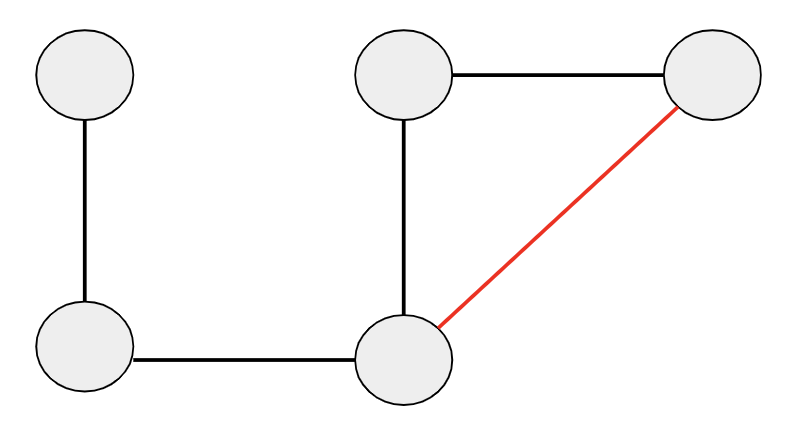
\includegraphics[scale=0.4]{images/strength.png}
\caption{Example graph illustrating edge strength}
\label{fig:ex_strong}
\end{figure}

Before we jump into how to use strength to determine the sampling probability, let's first introduce several useful lemmas. 

\begin{lemma}[Karger, et al \cite{benczur2015randomized}] \label{min_cut_exact_1}
In a connected graph G, suppose each edge e has strength $k_e$ and weight $w_e$, the graph $\hat{G}$ with the same set of edges and nodes but each edge e has weight $w_e/k_e$ will have minimum cut exactly 1.
\end{lemma}

To show that, suppose the minimum cut value in the original graph is c. For any edge in the original graph, its strength is at least c, given the entire graph is c-connected. For any edge in the minimum cut c, suppose it has strength k where k is larger than c, then it must be included in some subgraph $G_1$ with connectivity k. Thus any cut across this edge in $G_1$ will have value at least k, we can extend this cut by adding all nodes in $G - G_1$ into either side of the cut, then we constructed a cut in the original graph with value at least k, contradicts with c being the minimum cut. Thus we conclude every edge in the minimum cut c has strength value exactly c. 
Therefore the minimum cut value in $\hat{G}$ is 1. 

Figure \ref{fig:ex_strong} shows an example, the minimum cut consists of three edges $e_1$, $e_2$, $e_3$, all have edge strength $c = w_{e1} + w_{e2} + w_{e3}$, which is the minimum cut value, thus $w_{e1}/c + w_{e2}/c + w_{e3}/c = c/c = 1$.

\begin{figure}[h!]
\centering
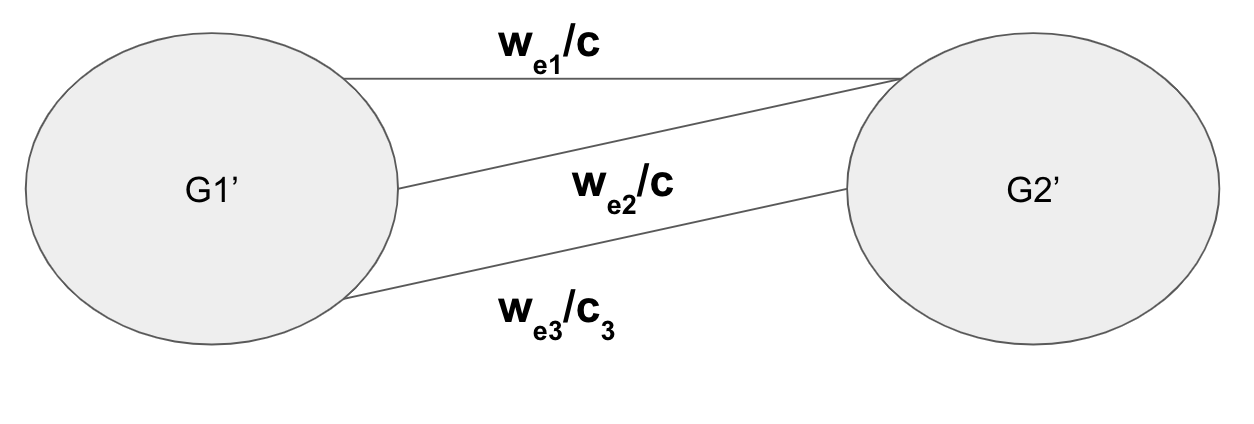
\includegraphics[scale=0.4]{images/mincut.png}
\caption{Example graph illustrating Lemma \ref{min_cut_exact_1}}
\label{fig:ex_strong}
\end{figure}

\begin{lemma}[Karger, et al \cite{benczur2015randomized}] \label{sigma_ue/ke}
In a weighted graph G, suppose each edge e has weight $u_e$ and strength $k_e$, then 
\begin{equation}
\Sigma u_e/k_e \leq n - 1
\end{equation}
\end{lemma}

This can be easily shown by induction. Suppose we have a graph $\hat{G}$ with the same set of vertices and edges as $G$ but each edge $e$ has weight $w_e/k_e$. It is trivially true for graph of only one node. Suppose this lemma is true for graph of $n_0$ vertices where $ 2 \leq n_0 < n$. We remove edges across minimum cut from graph $\hat{G}$, resulting in two connected components $G_1$ and $G_2$ with $n_1$ and $n_2$ vertices respectively where $n_1 + n_2 = n$. By our induction, the lemma holds for subgraph $G_1$ and $G_2$, thus
\begin{align}
    \begin{aligned}
        \Sigma_{e \in G_1} u_e/k_e + \Sigma_{e \in G_2} u_e/k_e 
        & \leq (n_1 - 1) + (n_2 - 1) \\
        & \leq n_1 + n_2 - 2 \\
        & \leq n - 2
    \end{aligned}
\end{align}

As shown in lemma \ref{min_cut_exact_1}, the minimum cut of $\hat{G}$ has value exactly 1, thus the lemma holds for a graph of size n.

\begin{lemma}[Karger, et al \cite{benczur2015randomized} \label{decomposition}]
A graph G can be decomposed into subgraphs of tree-structure. Any subgraph $K_i$ in the tree structure have strong-connectivity less than all of its successors and is a superset of any of its successors.
\end{lemma}

We can construct the tree structure recursively, the original graph $G$ is the root. Suppose its minimum cut value is $c$, we remove all edges with strength $c$, producing multiple subgraphs, and all the subgraphs are children of $G$. Notice that the strength of an edge in any of the subgraph is not affected after deleting those edges with strength $c$. Here is a simple proof argument: any edge remained will have strength larger than $c$, suppose it is $k$. It has to be inside some subgraphs $G_k$ that is k-strong by definition. On the other hand, for any edge $e$ with strength $c$, it must not be inside $G_k$. Thus deleting $e$ will not affect the strength of any remaining edge. We can recursively construct this tree structure such that it fulfills the definition. Figure \ref{fig:decomposition} has shown an example of the tree-structured sub-graphs. 


\begin{figure}[h!]
\centering
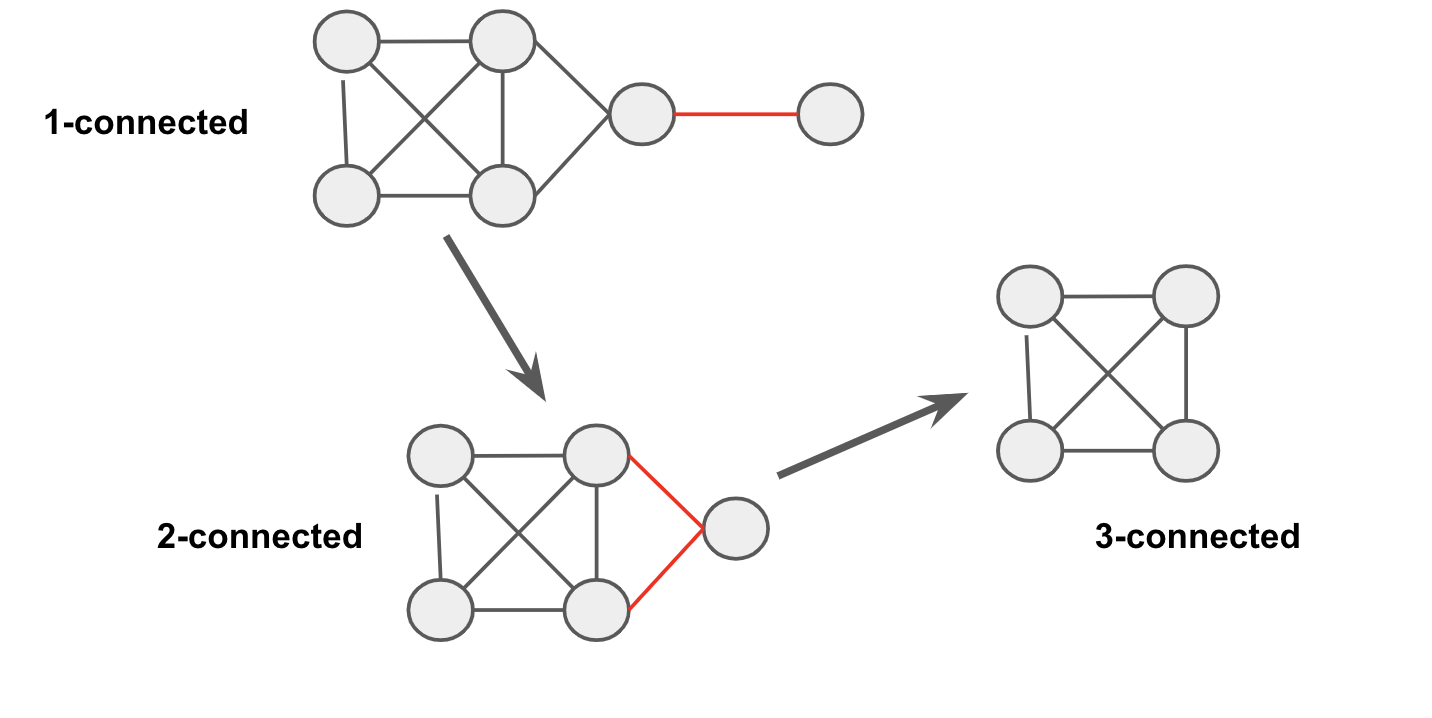
\includegraphics[scale=0.4]{images/decomposition.png}
\caption{Example graph illustrating Lemma \ref{decomposition}}
\label{fig:decomposition}
\end{figure}

\bigskip

Next, we show that if each edge is bounded by a certain factor of its strength, we can approximate the original $G$ by the weighted sum of approximation of all sub-graphs in the tree structure. To make the proof easier, the following alternative definition of Theorem \ref{theorem1} can be used. 

\begin{theorem}[Karger \cite{benczur2015randomized}] \label{theorem2}
Let $G$ be a graph in which edges have mutually independent random weights, each distributed in the interval [0, 1]. If the expected weight of every cut in G exceeds $3(d+2)(\frac{\ln{n}}{\epsilon^2})$, then with high probability every cut has value within $(1\pm\epsilon)$ of its expectation. 
\end{theorem}

Recall the tree-structure of $G$, consists of $r < n$ sub-graphs $G_1, G_2, G_3,..., G_r$, where sub-graph $G_i$ has strong-connectivity $k_i$. Let's define the parent of $G_i$ in the tree structure to be $G_{p_i}$, for each of the edge originally with weight $w_e$, let's give it weight $w_e' = cw_e/(k_e * p_e)$ where $k_e$ is the strength of edge $e$. $p_e$ and $c$ are some factors we decide later. We can express original graph by a weighted sum of those sub-graphs. 
\begin{equation}
    w_e = \Sigma ((k_i - k_{p_i}) / c) * w_e'* p_e
\end{equation}

It is easy to see that the series telescope, after simplifying, this series equals to $(k_e / c) * p_e * w_e' = w_e$. For each one of the sub-graph $G_i$, if we didn't multiply each edge's weight by $c/(k_e * p_e)$ but only $1/k_e$, then the minimum cut value is exactly 1 by lemma \ref{min_cut_exact_1}. Thus multiplying it by $c/(k_e * p_e)$ makes minimum cut to have value exactly $c/p_e$. Let's construct skeleton graph by sampling each edge with probability $p_e$, thus for each sub-graph $G_i$, it will have expected minimum cut value $(c/p_e) * p_e = c$. Let's choose $c = 3(d+3)(\frac{\ln{n}}{\epsilon^2})$, such that the expected weight of every cut in $G_1$ fulfill the requirements of Theorem \ref{theorem2}. It only remains to show that $cw_e/(k_e * p_e) \in [0, 1]$ (from here we can solve for $p_e$)such that we can directly apply Theorem \ref{theorem2} and get accurate approximation of cuts of each $G_i$ with high probability, and finally by union bound, we get accurate approximation of all cuts in $G$ with high probability. Notice this only holds if $cw_e/k_e \in [0, 1]$ for each edge $e$. Luckily there is an simple approach to make each edge satisfy this constraint, we can just split the edge with large weight into multiple parallel edges of smaller weight. 
\bigskip

To summaries the result from \cite{benczur2015randomized}, we can sample each edge with probability $p_e = min(1, cw_e/k_e)$,
where $c = 3(d+3)(\frac{\ln{n}}{\epsilon^2})$ and give weight $u_e/p_e$ if it is sampled, then with high probability, every cut in the $G$ will be within $(1 \pm \epsilon)$ times its expectation with high probability, and the skeleton graph has $O(nlogn)$ edges in expectation. To see that, notice the expected number of edges sampled = $\Sigma p_e = c\Sigma w_e/k_e = cn = O(nlogn)$ by lemma \ref{sigma_ue/ke}. 

\section{Estimate Edge Strength}
Notice the sampling scheme of the above section requires the knowledge of exact edge strength $k_e$ for every edge $e$, which is not easy to find out. Instead, we can try to estimate it. In this section, we will focus on how to estimate edge strength in \textbf{unweighted graph} in $O(m\log^2n)$ time. We will first look at what is our goal and what do we have. Then, we go through the steps to estimate the strength and improve the algorithm.

\subsection{What is our goal}
Our estimation strength $\hat{k_e}$ should satisfy the following two constraints: \\
1. For all edges, $\hat{k_e} \leq k_e$, where $k_e$ is the actual strength. \\
2. $\Sigma_{e} \frac{w_e}{\hat{k_e}} = \Sigma_{e} \frac{1}{\hat{k_e}} = O(n)$ (Noted that edge weight in unweighted graph is $1$) \\

The first constraint controls the sampling probability and edge weight assigned. With low estimated strength, the sampling probability will be higher and the weight assigned to edges in the skeleton graph will be smaller. We prefer more edges with small maximum weight to fewer edges with large maximum weight in our skeleton graph to have less variance of cut size in skeleton graph. 

The second constraint controls the number of remaining edges after sampling. Previously we derive that the number of edges in skeleton graph using actual strength $k_e$ is $c\Sigma 1/k_e \leq cn = O(n \log n)$, because $\Sigma 1/k_e \leq n - 1$. 
Now if we use estimated strength $\hat{k_e}$ given with the second constraint, the result is still asymptotically correctly

\subsection{What do we have}
We do not develop the algorithm from scratch. we have a black-box algorithm developed by Nagamochi and Ibaraki \cite{nagamochi1992linear} that can return all edges with standard connectivity $\leq k$. 
Formally, this set of edges is defined as a k-certificate, which means:
\begin{definition} [Sparse certificate, Karger, et al \cite{benczur2015randomized}]
A sparse k-certificate of graph G with n vertices is a subgraph H of G such that H has at most k(n-1) edges, and H contains all edges crossing cuts of value k or less.
\end{definition}
This algorithm, named as \textbf{$Certificate(G, k)$} can run in $O(m)$ time to compute a k-certificate on an unweighted graph. \\

However, note that this sparse certificate algorithm may not return some edges with \textbf{strong connectivity} $k_e \leq k$. 

As figure \ref{fig:ex_strong} shows, the red edge has strong connectivity 2. This is because each triangle is a subgraph with a min-cut size of 2, and there is no subgraph containing red edge with min-cut size 3.
However, its standard connectivity is 3, because any cut across the red edge is of size 3. Thus, if we call $Certificate(2)$, the red edge may not be returned, which is not what we want.

\begin{figure}[h!]
\centering
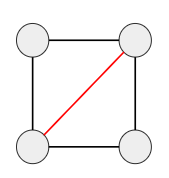
\includegraphics[scale=0.4]{images/square_example.png}
\caption{An example of certificate may not contain k-weak edges}
\label{fig:ex_strong}
\end{figure}

Thus, we have to modify the sparse certificate algorithm to get all k-weak edges.

\subsection{Find All k-weak Edges}
In the first step, we simply repeat querying \textbf{$Certificate(G, k)$} to get all k-weak edges.

\begin{algorithm}[H]
\SetAlgoLined

    \While{repeat $log_2n$ times} {
        $E' \gets Certificate(G, 4k)$\;
        
        \textbf{Output} $E'$\;
        
        $G \gets G - E'$\;
    }
        
\caption{WeakEdges($G$, $k$)}
\end{algorithm}

We claim that $Weak Edges(G, k)$ returns a set of edges containing all k-weak edges. 
To prove this, we first need a lemma that shows the number of k-weak edges is not too large.

\begin{lemma} \label{number_k_weak}
In a graph with n vertices, the number of k-weak edges is at most k(n-1).
\end{lemma}
Suppose not, let $S$ be the set of k-weak edges with size larger than $k(n-1)$, then

\begin{align}
    \begin{aligned}
        \Sigma u_e/k_e &\geq \Sigma_{e \in S} u_e/k_e \\
                       & > \Sigma_{e \in S} u_e/k \\
                       & > k(n-1)/k \\
                       & = n - 1
    \end{aligned}
\end{align}

This contradicts to Lemma \ref{sigma_ue/ke}. \\

Then, to prove that $Weak Edge$ returns all k-weak edges, we firstly consider a simple case that all edges are k-weak in graph $G$. 
By lemma \ref{number_k_weak}, $G$ has at most $k(n-1)$ edges. Then the total degree of $G$ is less than $2k(n-1)$, so at least half of vertices have degree less than $4k$. The red vertex in figure \ref{fig:ex_all_weak} represents such a vertex with degree less than $4k$.


\begin{figure}[h!]
\centering
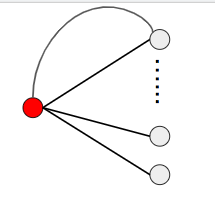
\includegraphics[scale=0.4]{images/all_weak_edge_example.png}
\caption{All edges are k-weak}
\label{fig:ex_all_weak}
\end{figure}

All edges connected to the red vertex will be returned by $Certificate(G, 4k)$ because putting it on one side and all other vertices on the other side will yield a cut value less than $4k$. Then, after removing all edges in a sparse certificate from the original graph, the red vertex will be isolated.
Therefore, at least half of vertices will be isolated after calling $Certificate(G, 4k)$, and removing returned edges. Since removing edges cannot increase the strength of other edges, the remaining edges will still be k-weak. Therefore repeating $\log n$ times will make all vertices being isolated, which means all edges are returned by $Weak Edge$, as desired. \\

\begin{figure}[h!]
\centering
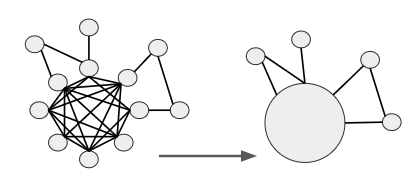
\includegraphics[scale=0.4]{images/contract_strong.png}
\caption{Contract k-strong Edges}
\label{fig:contract_strong}
\end{figure}

Then we consider a general graph. If an edge is k-strong, it should be contained in a sub-graph with min-cut size at least $k$ by definition. Therefore, all edges in that sub-graph must also be k-strong. Then we can contract all edges in that subgroup, resulting exactly one vertex shown in figure \ref{fig:contract_strong}.
If we do this for all k-strong edges, all remaining edges will be k-weak. Notice that removing k-strong edges will not affect the strength of k-weak edges. Therefore, a certificate in the graph after contraction is also a certificate of the original graph. Thus, the previous argument is still applicable for a general graph, and $Weak Edge(G, k)$ will return all k-weak edges in general graph.

\subsection{Strategy of Estimation}

Now $Weak Edge$ gives all k-weak edges. We will keep querying $Weak Edge(2^{k+1})$ and estimate all returned edges as $2^k$. Specifically, 
\begin{algorithm}[H]
\SetAlgoLined

    \For{$i \gets 1$ to $logn$} {
        $E_i \gets WeakEdge\_v2(G, 2^i+1)$\;
        
        \For{$e$ in $E_i$} {
            $\hat{k_e} \gets i$\;
        }
    
        $G \gets G - E_i$\;
    }
        
\caption{Estimate\_Strength($G$)}
\end{algorithm}

Thus, we first query $WeakEdge(2)$. The strength of all returned edges will be estimated as $1$, and they will be removed from the graph. Then we query $WeakEdge(4)$, estimate strengths of returned edges as $2$, and remove these edges from the graph. Repeat these steps until all edges have been estimated. Noted that the maximum possible strength of any edge is $n-1$.  

Recall that we have two requirements for estimation: \\
1. For all edge, estimated strength $\hat{k_e} \leq$ actual strength $k_e$ \\
2. $\Sigma_e \hat{k_e} = O(n)$ \\

It is easy to see that the first requirement is satisfied because $WeakEdge(k)$ guarantees to contain all k-weak edges. It is impossible to miss any edge $e$ when querying $WeakEdge(2^c)$ if $k_e \leq 2^c$.

However, note that the $WeakEdge$ algorithm only guarantees to contain all k-weak edges, and has no idea about how many k-strong edges it returns. 
If there are too many k-strong edges, we will underestimate the strength of these edges too much, and yield a bad estimator. Hence, we have to control the number of k-strong edges. 
The first version of $WeakEdges$ will return at most $4k(n-1)\log n$ edges, because each $Certificate(G, 4k)$ returns at most $4k(n-1)$ edges. 
In the worst case, all these edges could be k-strong, and thus we may underestimate them too much. 
Quantitatively, we get at most  $4*2^{i+1}(n-1)\log n$ edges in round $i$, and estimate their strengths as $2^i$. Then, 

\begin{align}
    \begin{aligned}
        \Sigma_{e} \frac{1}{\hat{k_e}} & = \Sigma_{i = 1}^{\log n} 4 \times 2^{i+1}(n-1) \log n \times \frac{1}{2^i} \\
       & = 8(n-1) \log^2 n \\
       & = O(n \log^2 n) \\
       & > O(n) 
    \end{aligned}
\end{align}
which does not satisfy the second requirement. \\

Therefore the first version of $Weak Edge$ is not good enough by querying sparse-certificate directly.

\subsection{Removing Redundant Edges in Certificate}

The next step is to remove some edges with standard connectivity larger than $k$ from the sparse certificate.
Firstly, there is a pattern of redundant edge: two endpoints of an edge in the certificate is connected by a path outside the certificate. For example, in figure \ref{fig:redundant_strong}, the three edges in the blue circle $E$ is a certificate. The endpoints of the red edge are connected by the green path, where all edges in that path are not in the certificate. Thus we claim that the red edge is redundant and can be removed from certificate safely.

\begin{figure}[h!]
\centering
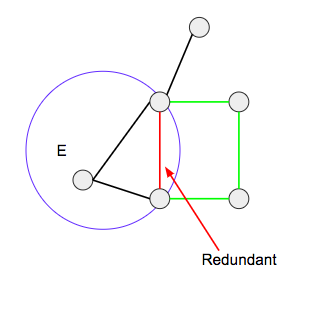
\includegraphics[scale=0.4]{images/redundant_edge.png}
\caption{Redundant k-strong edge in certificate}
\label{fig:redundant_strong}
\end{figure}

In general, suppose an edge $(u, v)$ is in a k-certificate $E$, while vertices $u$ and $v$ are connected by a path, and all edges in that path are not in $E$. Then $(u, v)$ has standard connectivity larger than $k$.
We know that all edges along the path are not across any cut smaller than $k$. 
Suppose $(u, v)$ has standard connectivity smaller than $k$, then there exists a cut with value less than k and cross $(u, v)$. Then this cut must separate $u$ and $v$, so an edge $e$ in the path that connects $(u, v)$ must also across the cut, contradiction.
Therefore $(u, v)$ can be safely removed from k-certificate $E$. \\

The way to remove such redundant edges from the certificate is that: after computing a certificate $E$ of graph $G$, we contract all edges in $G-E$ to generate a new graph $G'$. 
Note that removing edges with larger standard connectivity does not affect those edges with smaller standard connectivity, so all edges with smaller connectivity keep remained in $G'$. Therefore, finding a certificate in $G'$ still gets all k-smaller connectivity edges in the original graph. 
Since $G'$ has fewer vertices, the certificate of $G'$ will be more accurate and contain fewer redundant edges. Typically, if $G-E$ has $r$ connected components, $G'$ will have exactly $r$ vertices after contraction, so the number of k-smaller connectivity edges should be less than $k(r-1)$. In practice, we release it to $2k(r-1)$ for better running time. \\

Then, we have a better algorithm to find a certificate, named as $Partition$:

\begin{algorithm}[H] \label{partition_algo}
\SetAlgoLined
 Input: Graph with n vertices and m edges
    
    \eIf{$m \leq 2k(n-1)$}{
     Output edges in G\;
   }{
   $E \gets Certificate(G, k)$\;
   
   $G' \gets$ contract all edges of $G-E$\;
   
   Partition($G'$, $k$)\;
  }
        
\caption{Partition($G$, $k$)}
\end{algorithm}

As stated before, this $Partition$ algorithm is correct because removing strong connected edges does not affect weak edges. We want to show that  $Partition$ runs in $O(m+n)$ time. 

Since $m > 2k(n-1)$ is the condition to continue the algorithm, the certificate size $m'$ will satisfy $m' < k(n-1) < \frac{m}{2}$, and $G'$ has exactly $m'$ edges because all other edges in $G$ are contracted. Similarly, the number of vertices in $G'$, denoted as $n'$ must satisfy $n' > \frac{n-1}{2} + 1$. Otherwise $m' < k(n-1) < 2k(n'-1)$ will make it stop in next round. Therefore the size of both vertices and edges reduce by half for each recursion call. By master theorem, $T(m, n) = T(m/2, n/2) + m + n$ gives us running time $O(m+n)$

\subsection{Find k-weak Edges Tightly}
We now integrate $Weak Edge$ and $Partition$ to find all k-weak edges with fewer k-strong edges. 

\begin{algorithm}[H]
\SetAlgoLined

    \While{repeat $log_2n$ times} {
        $E \gets Partition(G, 4k)$\;
        
        \textbf{Output} $E$\;
        
        $G \gets G - E$\;
    }
        
\caption{WeakEdges\_v2($G$, $k$)}
\end{algorithm}

Notice that compared with the first version, $Weak Edge\_v2$ only replaces $certificate(4k)$ by $Partition(G, 4k)$, and the rest are all same.

It is clear that $Weak Edges\_v2$ runs in $O(\log n \times (m+n)) = O(m \log n)$ time. 

It is also clear that $Weak Edges\_v2$ returns a set $E$ containing all k-weak edges. 

We want to show that, suppose $G-E$ has $r$ connected components, size of $E$ is at most $8k(r-1)$. Since $Partition(G, k)$ will return $2k(a-1)$ edges which separate $G$ as $a$ connected components, $Partition(G, 4k)$ will return $8k(a-1)$ edges for $a$ connected components. Therefore every $8k$ edges will separate the graph for one more component, and $r$ components require $8k(r-1)$ edges.

\subsection{Estimate Edge Strength}
Now $WeakEdge\_v2$ gives all k-weak edges with limited k-strong edges. We use it to estimate the strength for each edge. 
\begin{algorithm}[H]
\SetAlgoLined

    \For{$i \gets 1$ to $logn$} {
        $E_i \gets WeakEdge\_v2(G, 2^i+1)$\;
        
        \For{$e$ in $E_i$} {
            $\hat{k_e} \gets i$\;
        }
    
        $G \gets G - E_i$\;
    }
        
\caption{Estimate\_Strength($G$)}
\end{algorithm}

Since the maximum strength of an edge is $n$, there are at most $logn$ outer loops. Hence, this algorithm runs in $O(logn \times (mlogn))$ = $O(mlog^2n)$ time. Then we prove the correctness of the algorithm.

Since $Weak Edge\_v2(G, k)$ guarantees to return all k-weak edges, the estimated strength still cannot exceed the actual strength. Then we focus on $\Sigma_{e} \frac{1}{\hat{k_e}} = O()$

Intuitively, the ideal situation is that for all edges with actual strength $k_e \in [2^k, 2^{k+1}]$, we estimate their strength as $\hat{k_e} = 2^k$. 
Therefore, each edge is underestimated at most half of its actual strength ideally. However, there still exist k-strong edges in the result of $WeakEdge\_v2$, but now the number of k-strong edges is under control.

We may treat $\frac{1}{\hat{k_e}}$ as costs of one edge, so the total costs of all edges should be bounded by the number of vertices.
Consider a subgraph $H$, after $WeakEdge\_v2(G, k)$ is called, a set $E$ of $8k(r-1)$ edges are returned and separate H as $r$ components, and these edges have estimation $\hat{k_e} = \frac{k}{2}$. Therefore, the edges in $E$ that separate original graph into $r$ components satisfy:

\begin{equation}
    \Sigma_{e \in E} \frac{1}{\hat{k_e}} = 8k(r-1) \times \frac{2}{k} = 16(r-1)
\end{equation}

As the number of connected components increases from $1$ to $r$, edges that separate each extra components contribute 16 units of costs on average.
In the end, all edges are removed and we have $n$ components, resulting in $n-1$ extra connected components. Apply the equation above, the total costs will be $16(n-1)$. Therefore, 

\begin{equation}
    \Sigma \frac{1}{\hat{k_e}} = 16(n-1) = O(n)
\end{equation}

as desired.

In conclusion, the strength of all edges in an unweighted graph can be estimated in $O(m \log^2 n)$ time.

\section{Extensions}
In this section, we focus on two extensions: experiments on replacing strong connectivity by standard connectivity, and streaming algorithm for sampling if we are unable to store the original graph. \\

In the latest version of the publication \citep{benczur207078randomized}, the authors state that although the concept of \textbf{strong connectivity} is introduced to make the algorithm work, there is no counterexample showing that using the \textbf{standard connectivity} in the algorithm will make it failed. Therefore, our first extension is to run experiments to study the accuracy of the algorithm if we use the standard connectivity in replace of strong connectivity in sampling. \\

The second extension, which is theoretical, is based on the situation that the original graph is too large to be stored, but new edges will be added gradually. We have proposed a streaming algorithm for unweighted graphs that can update the skeleton graph when new edges are introduced. However, this algorithm is based on the assumption that standard connectivity instead of strong connectivity can be used for sampling, which has not been proved or disproved so far.

\subsection{Experiments}

In this section, we will implement the sampling algorithm based on standard connectivity, and run experiments on several types of graphs which are typical to determine the performance of replacing strong connectivity by standard connectivity. \\

An easy observation we can make is that the standard connectivity of an edge is always as big as its strong connectivity. Suppose its strong connectivity is $k_e$, by definition, we know that there must exist some $k_e$ connected sub-graph $G'$ that contains this edge. Consider any cut that separates this edge's endpoints, it must also separate $G'$. In other words, the cut needs to be at least of size $k_e$. One typical case where standard connectivity gets bigger than strong connectivity is that when there exists a path connecting two endpoints of the edge, and none of the edges along the path is inside the k-connected sub-graph. Figure \ref{fig:StandardC} shows an example. The sub-graph inside the blue circle is a 3-connected sub-graph, and all edges of that sub-graph have strong connectivity of 3. However, the endpoints of the red edge are connected by a path outside that sub-graph, marking as green lines. The standard connectivity of the red edge is 4, which is larger than its strong connectivity. \\

\begin{figure}[h!]
\centering
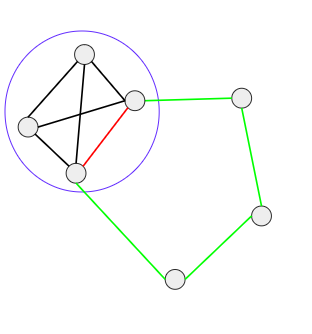
\includegraphics[scale=0.4]{images/standard_bigger_strong.png}
\caption{Extra path outside sub-graph}
\label{fig:StandardC}
\end{figure}

Therefore, by using standard connectivity, our sampled graph could be potentially sparser than that using strong connectivity, because the larger standard connectivity will result in lower sampling probability.

\subsubsection{Implementation}
The first step of our experiment is to estimate each edge's standard connectivity, and our implementation is the following:

\begin{algorithm}[H]
\SetAlgoLined

    \For{$i \gets 1$ to $\log n$} {
        $E_i \gets Partition(G, 2^i+1)$\;
        
        \For{$e$ in $E_i$} {
            $\hat{k_e} \gets i$\;
        }
    
        $G \gets G - E_i$\;
    }
        
\caption{Estimate\_Edge\_Connectivity($G$)}
\end{algorithm}

The $Partition$ algorithm is the one in section \ref{partition_algo}, and we have also implemented the $Certificate$ function inside $Partition$ algorithm, referred to Nagamochi's algorithm \cite{nagamochi1992linear}.

\bigskip

Next, we follow the basic mechanism of non-uniform sampling as we have introduced in section 3, except we use standard connectivity to replace strong connectivity. \\

\subsubsection{Interested Properties}
To examine the performance of the algorithm, we are interested in two properties: \textbf{compression rate} and \textbf{accuracy}.
We first compute the compression rate of the sampling, which is defined by the ratio of edge numbers between the skeleton graph and the original graph. Formally, if there are $m$ edges in the original graph and $m'$ edges in the skeleton graph, then the compression rate will be:

\begin{equation}
    compression\_rate = \frac{m'}{m}
\end{equation}

Therefore, a low compression rate implies that the skeleton graph is sparse, which is what we want. \\

Then, we compute the accuracy of the skeleton graph. We use the s-t minimum cut to measure the cut size.
We randomly select a set of pairs of vertices $E$ from the original graph. For each pair of vertices in $E$, we compute its s-t minimum cut in both the original graph and skeleton graph. Suppose the pair of vertices has s-t minimum cut size $c_e$ and $c'_e$ in the original graph and skeleton graph, respectively. The accuracy of this pair will be $ 1- \frac{|c'_e - c_e|}{c_e}$. Its maximum value $1$ implies that min cut in the skeleton graph is exactly the same as that in the original graph. Then we compute the average accuracy of all pairs of vertices in $E$ and use this value to estimate the accuracy of the skeleton graph, which is formally written as:

\begin{equation}
    accuracy = 1 - \frac{1}{|E|} \Sigma_{e \in E} \frac{|c'_e - c_e|}{c_e}
\end{equation}

Therefore, high accuracy implies the cut value in the skeleton graph is well-preserved, which is what we desire. \\

Our overall strategy is to tune the tolerance rate $\epsilon$. Recall that the sampling probability $p_e = \frac{(d+2) \times \ln{n}}{\epsilon^2 \times k_e}$, where $d$ is constant, and $k_e$ is the estimated standard connectivity. Therefore, tuning tolerance factors will affect the sampling probability, and thus changes the compression rate. \\

Finally, we will find out the relationship between compression rate and accuracy. Since now we are using standard connectivity instead of strong connectivity for sampling, the accuracy could decrease when the compression rate decreases. Therefore, we also want to determine how significantly the accuracy decreases when the compression rate decreases. 
\bigskip

\subsubsection{Experiment on Star-Clique Graph}
The star-clique graph is constructed by connecting a group of cliques to a central node. An example is shown in Figure \ref{fig:StarClique}, where 4 cliques each with 4 nodes are connected by the center node. Typically, a star-clique graph have minimum cut value exactly $1$, each edge incidents on the center node have standard connectivity $1$, and each edge inside any clique has standard connectivity $k$ where $k$ is the number of nodes in that clique.

\begin{figure}[h!]
\centering
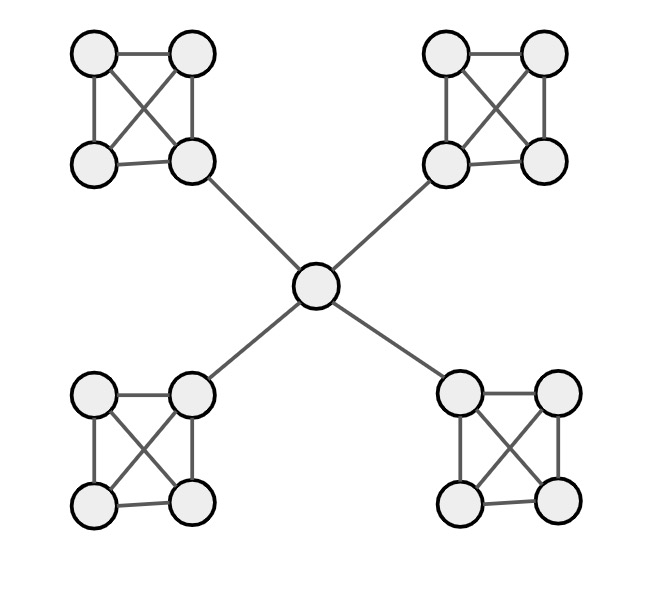
\includegraphics[scale=0.2]{images/starClique.jpg}
\caption{An example of Star-Clique Graph}
\label{fig:StarClique}
\end{figure}

\begin{tikzpicture} 
\label{clique_result}

\begin{axis}[
    xlabel={Compression Rate},
    ylabel={Accuracy},
    xmin=0, xmax=0.5,
    ymin=0.85, ymax=1,
    xtick={0,0.1,0.2,0.3,0.4,0.5},
    ytick={0.85,0.88,0.91,0.94,0.97,1},
    legend pos=north west,
    ymajorgrids=true,
    grid style=dashed,
]

\addplot[
    color=blue,
    mark=square,
    ]
    coordinates {
(0.4693720530379782,0.9564)(0.3003266174546431,0.9306)(0.20868569385306307,0.8816)(0.1534105818006833,0.8772)(0.11751156992522133,0.862)  
    };
\end{axis}
\end{tikzpicture}

The figure above shows the result of the star-clique graph with 10 cliques, and each one has 1500 nodes. The accuracy decreases when the compression rate decreases, as we expected. The estimation of the cut with a size $1$ in the original graph, as the algorithm guarantees those edges with a minimum cut size of $1$ can be estimated correctly. However, the cuts inside a clique may have a larger variance, because high connectivity implies low sampling probability and the large weight assigned, which make the variance large. However, the overall accuracy is high, probably because most edges in the star-clique graph has the same value of standard connectivity and strong connectivity.

\subsubsection{Experiment on Uniform Random Graph}
Next, we have run the experiment on a randomly generated graph. We choose each edge by selecting its two endpoints randomly. In other words, each of the $n \choose 2$ edges has an equal chance of being chosen. Therefore, the graph should have a uniform density across all parts, and all cuts should have a similar size in expectation. An example of a uniform graph shown in figure \ref{fig:unifrom_graph} has similar densities among all parts, and the standard connectivity of all edges are similar.

\begin{figure}[h!]
\centering
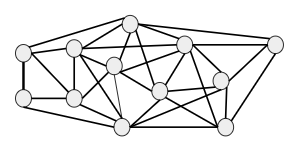
\includegraphics[scale=0.5]{images/uni_graph.png}
\caption{An example of uniform graph}
\label{fig:unifrom_graph}
\end{figure}

\begin{tikzpicture} \label{uniform_graph}
\begin{axis}[
    xlabel={Compression Rate},
    ylabel={Accuracy},
    xmin=0, xmax=0.6,
    ymin=0.86, ymax=1,
    xtick={0,0.1,0.2,0.3,0.4,0.5},
    ytick={0.85,0.88,0.91,0.94,0.97,1},
    legend pos=north west,
    ymajorgrids=true,
    grid style=dashed,
]

\addplot[
    color=blue,
    mark=square,
    ]
    coordinates {
(0.5112389,0.988374)(0.338302, 0.959031)(0.2396382,0.933029)(0.1775176, 0.902858)(0.1370506, 0.886064)  
    };
\end{axis}
\end{tikzpicture}

We have run our experiment on a uniform graph with 10000 nodes and 10000000 edges, as we can see from the figure when compression rate goes down, that means we compressed more edges, the accuracy of the estimation also goes down, which is expected. Using standard connectivity in uniform random graph seems to work well.

\subsubsection{Experiment on Non-uniform Random Graph}
Finally, we construct a graph with different densities across different sub-graphs. Specifically, we construct some uniform dense graphs and some uniform sparse graphs, connecting them with some edges to produce the final graph. As an example in figure \ref{fig:non_unifrom_graph}, the left part is sparse while the right part is dense. We connect them by the six red edges and form a non-uniform random graph.

\begin{tikzpicture} \label{swap_graph}
\begin{axis}[
    xlabel={Compression Rate},
    ylabel={Accuracy},
    xmin=0, xmax=0.7,
    ymin=0.86, ymax=1,
    xtick={0,0.1,0.2,0.3,0.4,0.5},
    ytick={0.85,0.88,0.91,0.94,0.97,1},
    legend pos=north west,
    ymajorgrids=true,
    grid style=dashed,
]

\addplot[
    color=blue,
    mark=square,
    ]
    coordinates {
(0.62383457246,0.971905)(0.433233049, 0.966448)(0.3184017144,0.960662)(0.24391766286, 0.926523)(0.192611498, 0.886064)  
    };
\end{axis}
\end{tikzpicture}

In this experiment, we combined 13 graphs each with different density to obtain the combined graph. Thus the cut values are no longer uniform, cuts in different sub-component will have different values. As we can see from the figure, we get similar results as compared to a uniform graph.

\begin{figure}[h!]
\centering
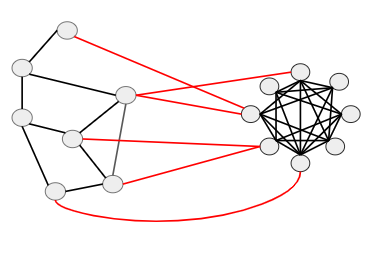
\includegraphics[scale=0.4]{images/non_unifrom_graph.png}
\caption{An example of non-uniform graph}
\label{fig:non_unifrom_graph}
\end{figure}

In all the three types of graph, we have experimented with, using standard connectivity seems to be working pretty well. It is possible that using standard connectivity is enough in doing sampling, which remains to be an open question. However, one conjecture is that standard connectivity and strong connectivity cannot deviate too much in the graph overall, there might be some bounded relationship between standard and strong connectivity, which also remains to be an open question.

\subsection{Sampling with Streaming Model in Unweighted Graph}
So far we have been assuming that the original graph does not change over time, which might not be the case in the real world. Here we consider a small problem where for an unweighted graph: a small set of new edges will be added to the graph without introducing new vertices. Do we have to sample the entire graph again? What if the original graph is no longer available?

\bigskip

To answer these questions, first notice the standard and strong connectivity of an existing edge can only increase because of the new added edges, which simply indicates for some of the existing edges, we should have sampled them with a lower probability than we have done. This means that the current sampling of existing edges can still yield good estimation with high probability, even though it might contain a bit more edges than we expected. Therefore, we could just focus on how to sample the new added edges. If the original graph is available, the question becomes easy, we may just estimate the new added edges' strong or standard connectivity in order to sample them. A more interesting case is that when the original graph is not available, we need to find some information useful from the skeleton graph.

\bigskip

It is not clear how can we find the new added edges' strong connectivity of the original graph from the sampled graph. because each edge in the sampled graph is weighted and the weight is related to its strong connectivity in the original graph. However, if we assume that we can use standard connectivity instead of strong connectivity, we can find the estimation of new added edges' standard connectivity of the original graph from the sampled graph. Recall that the sampled graph has all cut values within a factor of $\epsilon$ from expected with high probability. Thus, for any edge, the standard connectivity does not deviate by more than a factor of $\epsilon$ with high probability. Suppose each edge is added one at a time. For each newly added edge $e$ with two endpoints $s$ and $t$, before we flip a coin and decide whether to include it in our sampled graph, we first find the $s-t$ minimum cut value $h$ in the sampled graph using any classic $s-t$ minimum cut algorithm. Suppose the new edge's standard connectivity in the original graph (which is what we want to estimate) is $k_e$. Thus its weight in the sampled graph should be $w_e = \frac{k_e}{c}$ if sampled, where $c = 3(d+3)(\frac{\ln{n}}{\epsilon^2})$ as shown in section 3. \\

Combining them yields the following equations:

\begin{align}
    \left\{
        \begin{aligned}
            k_e &= h + w_e \\
            w_e &= \frac{k_e}{c}
        \end{aligned}
    \right.
\end{align}

By solving this we can have $k_e = \frac{1-c}{c}h$. Then, we add this edge into the sampled graph with probability $\frac{k_e}{c}$, and assign it weight $\frac{c}{k_e}$  if it is included. Since $h$ does not deviate from expectation by a factor of $\epsilon$ with high probability, the same goes for $k_e$. Since we did not update the existing edge, the expected standard connectivity could be slightly smaller than actual, but again, underestimation does not hurt us. For each newly added edge, with high probability, let's say at least $1- \frac{1}{n^d}$ for some constant $d$, we get the right estimation of its standard connectivity. Suppose we add $\alpha$ edges, we know $\alpha \leq n^2$ as no new vertex is introduced. Then taking the union bound, the probability $P$ that we sample all edges successfully will be: 

\begin{align}
    \begin{aligned}
        P &\geq 1 - \frac{1}{n^d} \times \alpha
          &\geq 1 - \frac{n^2}{n^d}
          &\geq 1 - \frac{1}{n^{d-2}}
    \end{aligned}
\end{align}

Thus all edges can be successfully sampled with high probability.\\

Notice this scheme only works well for a small set of new added edges, if we add a large number of edges, we could still get the right estimation, however, we might as a result lose the bound on $O(n \log n)$ number of edges and have a dense sampled graph, because we did not update existing edge's weight when its standard connectivity increases due to new added edges.


\section{Conclusion}
To summarize, we have first introduced an uniform sampling scheme in which we sample each edge with probability $p = \theta (\frac{\ln{n}}{\epsilon^2c})$ where $c$ is the minimum cut of the graph, therefore it does not work so well when the graph has a small minimum cut but is actually dense. Thus a non-uniform sampling method has been introduced where we sample each edge with probability relates to its strength. By doing so, we successfully reduced the number of edges in the sampled graph to $O(n \log n)$(independent of minimum cut value) and precisely preserving all cuts with high probability. The last question is how can we find out the strength of each edge. We want to find a good algorithm that can approximate the strength of each edge $k_e$ in the graph. We repeat a black-box algorithm that can return a k-certificate several times to get all k-weak edges. Then we contract all edges not in the certificate to control the number of k-strong edges returned by the algorithm. Finally, we can estimate all edges with actual strength within the range $[2^k, 2^{k+1}]$ to be $2^k$, and this turns out a good estimator that satisfies our requirement. \\

We have run experiments to explore whether using standard connectivity in replace of strong connectivity during sampling could still yield good estimation. We have chosen three types of typical graph and they all seem to be living well with standard connectivity. Lastly, we have discussed a streaming model where a new set of edges being added while the original graph is no longer available, we have shown that we can find estimation of the standard connectivity in the sampled graph, and sample them using that standard connectivity could give us a new sampled graph that still yields good estimation, even though it might contain more edges than we expected because we never modify existing edges' standard connectivity.

\bibliographystyle{plain}
\bibliography{references}
\end{document}
